% Template for Cogsci submission with R Markdown

% Stuff changed from original Markdown PLOS Template
\documentclass[10pt, letterpaper]{article}

\usepackage{cogsci}


\title{Modeling Selection in Active Cross-situational Word Learning}

\cogscifinalcopy

\author{{\large \bf George~Kachergis (kachergis@stanford.edu)} \\ Department of Psychology, Stanford University \\ Stanford, CA \AND {\large \bf Martin~Zettersten (mzettersten@ucsd.edu)} \\ Department of Cognitive Science, University of California, San Diego \\ San Diego, CA}


\begin{document}

\maketitle

\begin{abstract}
Word learning is a complex, interactive process, in which learners do
not passively observe a stream of words and referents, but are rather
actively involved in selecting referents and directing their attention
-- both of which are likely determined by their current knowledge state.
Thus, understanding how learners actively select information during word
learning can reveal the cognitive mechanisms underlying language
acquisition. The present study reanalyzes data from Zettersten \&
Saffran (2021), in which adults and children (ages 3-8) learned novel
word-referent mappings through cross-situational learning, then selected
which referents to receive additional training on. Participants'
individual training data, selection choices, and test trials were used
to fit four associative word learning models, and to infer the most
likely of five sampling strategies. Models with a bias to attend to
stimuli with uncertain (i.e.~high-entropy) knowledge states best
accounted for the data, though there were individual differences in the
degree to which this bias appeared to be the main driver of learning.
Approximately half of participants appear to be driven solely by this
bias (51\%), while another 48\% were best accounted for by a model
additionally engaging a competing familiarity bias. Analysis of
selection strategies revealed both developmental consistencies and
differences: while adults and children predominantly use an information
gain strategy to reduce uncertainty about ambiguous items, adults
deployed more diverse strategies (confirmatory, margin, and random
sampling). These findings suggest that reducing uncertainty can drive
sampling behavior even in young children, but that the repertoire of
sampling strategies grows with maturity. Moreover, individual
differences in learning mechanisms---particularly learning rate and
memory---are more predictive of word learning success than sampling
strategy alone.

\textbf{Keywords:}
active learning; cross-situational word learning; self-directed
learning; uncertainty reduction
\end{abstract}

\section{Introduction}\label{introduction}

Early word learning is often viewed as largely determined by the
learner's linguistic environment, where acquisition is constrained by
what is present in the input. Increasingly, however, research reveals
that learners--even young children--actively select and shape their
input, and that such self-directed learning can accelerate acquisition
(Smith et al., 2018; Twomey \& Westermann, 2018). Understanding the
strategies learners use to curate their experience can advance theories
of language acquisition, reveal the cognitive mechanisms and capacities
available across development, and inform the design of educational
curricula that match learners' expanding capabilities.

Despite growing interest in active learning, most computational models
of word learning have been evaluated exclusively on passive
cross-situational learning paradigms, in which participants observe
ambiguous training trials presenting multiple word-referent pairs
without indication of the correct mappings (Kachergis et al., 2017; Yu
\& Smith, 2007). While model comparisons in these passive contexts are
informative, active learning paradigms in which learners control some
aspect of their input (e.g., selecting which item to learn about next)
can be more diagnostic of underlying learning mechanisms and may better
capture individual differences in learning success (Gureckis \& Markant,
2012; Markant et al., 2016). Yet few active word learning experiments
have been conducted, and fewer still have attempted to explain active
learning behavior with computational models (though see Kachergis et
al., 2013).

The goal of the current study is to test how well associative models can
explain both learning outcomes and information-seeking during
cross-situational word learning, identify what sampling strategies
learners pursue, and track how sampling strategies develop with age. To
investigate these questions, we model data from a set of active,
cross-situational word learning experiments with children and adults
(Zettersten \& Saffran, 2021). In these experiments, adults
preferentially selected items with ambiguous word-referent mappings
during a sampling phase, while children (ages 3-8) increased their
preference to sample ambiguous items across age. We address three main
questions: First, which model architecture best captures individual
learning performance? Second, do specific model parameters (learning
rate, memory decay, attention to uncertainty) predict learning success?
Third, what sampling strategies (e.g., entropy reduction
vs.~confirmatory sampling) best explain participants'
information-seeking choices, and how do these strategies develop with
age? To address these first two issues, we chose a family of models that
instantiate trial-by-trial associative learning with memory decay and
selective attention to familiar and/or uncertain (or novel) stimuli,
which have been shown to account well for semantic bootstrapping and
mutual exclusivity effects in prior work (Kachergis et al., 2012, 2017).
To answer the third question, we subsequently used the best-fitting
models of participant learning to investigate which of a range of
decision rules best accounted for individuals' sampling choices.

Understanding children's and adults' sampling strategies during word
learning has important implications for theories of vocabulary
development. Past work shows that both children and adults actively seek
information about word meanings (Hembacher et al., 2020), which may help
explain rapid vocabulary growth (Hidaka et al., 2017). However, we lack
a formal understanding of the specific decision rules governing when
learners seek new information versus consolidate existing knowledge
(Settles, 2012; though see Gelderloos et al., 2020; Keijser et al.,
2019). Recent developmental work documents broad changes in
information-seeking strategies across childhood in domains such as
causal learning (Nussenbaum et al., 2020) and foraging (Meder et al.,
2021; Nussenbaum et al., 2023), suggesting that strategic sampling may
emerge gradually across development. The current work therefore explores
what sampling decision rules best explain children's and adults'
information-seeking during word learning, and how learning mechanisms
relate to sampling strategies.

A final important theoretical question concerns the relationship between
learning success and sampling strategy. Zettersten \& Saffran (2021)
found that adults who sampled more ambiguous items during the selection
phase showed higher test accuracy. However, the directionality of this
relationship remains unclear: does sampling ambiguous items \emph{cause}
better learning, or does successful learning \emph{enable} more
sophisticated ambiguity-seeking strategies? Their supplementary analyses
suggested the latter: as participants became more successful at learning
during training, they became more likely to seek information about
ambiguous items. We investigate this question by examining whether
individual differences in learning parameters (learning rate, memory,
attention biases) predict both test performance and sampling strategy,
potentially illuminating the mechanisms linking learning capacity to
active information-seeking.

\section{Method}\label{method}

\subsection{Data}\label{data}

All data were taken from Zettersten \& Saffran (2021). Data from
Experiment 1 (31 adults), Experiment 2 (40 children, 4-9 years of age),
and adults in the Ambiguous Condition of Experiment S1 (58 adults) were
pooled, as they all had the same design, except for an additional test
before the selection phase in Exp. S1. The training phase of these data
contained 24 trials, each comprised of 2 referents and 2 words. The
particular words and referents involved in each pairing were randomized
per participant, but the same training trial sequence--and thus
co-occurrence statistics--were experienced by all participants.
Experiment 3, with data from 58 children, 3 to 8 years of age, had a
similar design, except that two of the word-referent pairs were already
familiar to children (``dog'' and ``pig''). All of the experiments
followed the same training-sampling-test design: after a training phase
in which participants were exposed to referent-word co-occurrences,
participants had the opportunity to select which object they would learn
about next (sampling phase), followed by a test phase in which they were
asked to identify the referent of each word.

Sampling trials for kids differ slightly from adults in that there was
no random label-referent pair given: thus, the evidence children
received after selection was unambiguous, while adults received a
training trial with a randomly-selected label and its corresponding
referent. The models will see what the learner saw: for children, that
would be an unambiguous trial with the selected referent and its label;
while for adults, the model will be presented with the selected stimulus
pair alongside the random pair the learner saw.

\subsection{Models}\label{models}

We focused on analyzing data from the familiarity- and
uncertainty-biased associative model (Kachergis et al., 2012, 2017), and
variations of that model, described below. We chose not to test any
hypothesis-testing (HT) model as they are not consistent with the adult
data in Zettersten \& Saffran (2021): for ambiguous items in the
training phase, there was never any disconfirming evidence, so a
hypothesis-tester's initial guess (i.e.~hypothesis) for each label would
be confirmed on subsequent appearances, and there would be no reason for
(or basis for) preferentially selecting ambiguous referents during the
sampling phase, which is what adults were observed to do. While it is
possible that children -- who were at chance for selecting ambiguous
vs.~unambiguous referents -- are employing a hypothesis-testing
strategy, some of the selection strategies we want to evaluate across
development are only possible to use if a learner is simultaneously
entertaining multiple hypotheses for a given label -- equivalent to
associations rather than the mutually-exclusive hypotheses favored in HT
accounts (e.g. Woodard et al., 2016).

\subsubsection{Familiarity- and Uncertainty-biased Associative Model
(FUAM).}\label{familiarity--and-uncertainty-biased-associative-model-fuam.}

The FUAM assumes that learners accumulate associations between all
presented words and referents on each trial, but that their attention is
biased more towards particular word-referent associations on the basis
of prior experience. In particular, more attention (i.e.~associative
weight) is directed to associations between words and referents that
have appeared together on earlier trials (i.e., a familiarity bias). In
addition, more attention is directed to stimuli that have higher
uncertainty (i.e.~entropy, \(H\)) in their associations, whether because
they are novel (and thus have no pre-existing associations) or because
they have diffuse associations with several different stimuli. The model
assumes learners knowledge grows trial-by-trial, and that a fixed amount
of associative weight (learning rate \(\chi\)) is distributed among the
presented word-referent associations on a given trial in proportion to
the prior familiarity of the association and the uncertainty of the
involved word and referent. The relative strength of the familiarity and
uncertainty bias is governed by a parameter \(\lambda\): for values of
\(\lambda>1\) the model focuses more attention on uncertain stimuli,
while for values of \(\lambda<1\) the model focuses more attention on
familiar word-referent associations. Associations are also assumed to
decay from trial to trial, at a rate governed by memory fidelity
parameter \(\alpha\). The update rule for adjusting the association
\(M_{w,o}\) between word \(w\) and referent \(o\) on a given trial is

\begin{equation}
M_{w,o} =  \alpha M_{w,o} + \frac{ \chi \cdot e^{ \lambda \cdot (H(w) + H(o)) } \cdot M_{w,o}  }{  \sum_{w\in W} \sum_{o\in O} e^{ \lambda \cdot (H(w) + H(o)) } \cdot M_{w,o} }
\label{eq:fullmodel}
\end{equation}

When tested on word \(w\), the model assumes learners choose referent
\(o\) from the offered alternatives in proportion to their associative
strength \(M_{w,o}\) (i.e., Luce choice). The other models we tested are
variations on this model.

\subsubsection{Familiarity-biased Associative Model
(FAM).}\label{familiarity-biased-associative-model-fam.}

The familiarity-biased associative model (FAM) implemented just the
familiarity bias of the FUAM, without the uncertainty bias term, and
thus only implements a bias for already-strong associations, using
learning rate (\(\chi\)) and decay (\(\alpha\)) parameters.

\subsubsection{Uncertainty-biased Associative Model
(UAM).}\label{uncertainty-biased-associative-model-uam.}

The uncertainty-biased associative model (UAM) implemented only the
uncertainty bias of the FUAM without the familiarity bias term, and uses
the same three parameters as the FUAM.

\subsubsection{Novelty-biased Associative Model
(NAM).}\label{novelty-biased-associative-model-nam.}

The novelty-biased associative model (NAM), like the UAM, has no
familiarity bias, but instead of the entropy terms (\(H(w)\) and
\(H(o)\)) uses novelty (e.g., \(1/(frequency(w)+1)\)).

\subsection{Fitting Procedure}\label{fitting-procedure}

We first fitted each model to each participant's data individually,
finding parameter values per participant to maximize the log-likelihood
of the model's choices with respect to theirs. We fitted each model to
just the passive training trials, as well as to the passive training
trials and the participant's selection trials, to confirm that including
the selection trials yielded a better fit. We will report each model's
average fit, and select the best-fitting model overall for further
analysis.

\subsection{Modeling Sampling Choices}\label{modeling-sampling-choices}

Next, we used the best-fit models of participants' learning to
investigate their selection strategies in the sampling phase of the
experiment. Our goal was to evaluate two main sampling decision rules
commonly attested in the information-seeking literature to explain
active choices: maximizing entropy reduction (information gain) and
margin sampling. We also investigated three additional decision rules
(confirmatory, novelty-based, and random choices) to gain a full picture
of possible sampling strategies.

\subsubsection{Maximizing entropy
reduction.}\label{maximizing-entropy-reduction.}

In this decision rule, the model's goal is to maximally reduce the
entropy of the object-label probability distribution across objects
(Nelson, 2005; Settles, 2012). Sampling choices are modeled by comparing
the relative entropy reduction provided by making a given sampling
selection of a referent \(s_o\) (across the labels \(w\)):

\begin{equation}
\max_{s_o,w}({H(w)-H(w|s_o)})
\label{eq:entropy_reduction}
\end{equation}

Modeling selections were made by determining, on any given trial for a
participant, which object maximally reduced entropy (averaging across
all possible random distractors that could be chosen in the case of the
adult data).

\subsubsection{Margin sampling.}\label{margin-sampling.}

An alternative strategy documented is focusing on reducing uncertainty
for a more constrained set of items (Markant et al., 2016). This
strategy can be formalized as \emph{margin sampling}, in which the model
focuses only on the boundary between two alternative options. Margin
sampling predicts that learners will focus on instances where there is
highest ambiguity between the two most likely labels for a given
referent. Formally, if the distribution of labels
(\(\{l_1,l_2,...,l_n\}\)) for a given referent \(o\) are ordered from
most (\(p_1\)) to least (\(p_n\)) likely, \(\{p_1,p_2,...,p_n\}\), the
margin between labels is given by

\begin{equation}
LM(x) = 1 - (p_1 - p_2)
\label{eq:margin_sampling}
\end{equation}

In other words, the model selects the object that has the greatest
ambiguity or competition between its two strongest associates.

\subsubsection{Alternative strategies.}\label{alternative-strategies.}

We also tested a few additional strategies. First, we considered a
\emph{maximum certainty} (or \emph{confirmatory}) strategy. Learners may
gravitate towards confirming choices they already have high certainty
for (Wason, 1960; Zettersten et al., 2023; Zettersten, Chen, et al.,
2025). Second, we considered a \emph{novelty-based} strategy in which
the model based its choices on the relative novelty (or familiarity) of
the choice options. Third, we consider a \emph{random} selection
strategy as a baseline comparison.

\section{Results}\label{results}

\begin{table}[H]
\centering
\begin{tabular}{lrrrrr}
  \hline
Model & N best fit & Fam & Unc & Nov & FUAM \\ 
  \hline
FUAM &  67 & 1.66 & 1.66 & 1.65 & 1.42 \\ 
  Fam &  24 & 2.00 & 2.09 & 2.00 & 2.00 \\ 
  Nov &   3 & 3.22 & 3.42 & 3.01 & 3.19 \\ 
  Unc &  96 & 3.56 & 2.57 & 3.49 & 3.37 \\ 
   \hline
\end{tabular}
\caption{Number of participants best fitted per model, and average negative log-likelihood (lower=better) per model.} 
\end{table}

For all four models, including the selection trials yielded a better fit
to the data, showing that it is not unreasonable to apply these models
to the selection trials, and supporting the idea that the model's
knowledge state and parameters may bear some relation to participants'
selection strategies. For model comparison, we calculated BIC (Bayesian
Information Criterion), defined as \(BIC=ln(N)k-2ln(L)\), where \(L\) is
the maximized likelihood, \(k\) is the number of parameters, and \(N\)
is the number of data points (here, \(N=1712\) test trials). The model
with the lowest BIC is selected, as it balances model complexity and fit
to the data. The familiarity-biased model yielded \(BIC = 1036.17\), the
novelty-biased model scored \(BIC = 1026.68\), and the familiarity- and
uncertainty-biased model (FUAM) had \(BIC = 975.22\). The
uncertainty-biased model (UAM) yielded the best fit, with
\(BIC = 859.09\). Recognizing that different participants may be
operating under different learning regimes, we opted to investigate how
many participants were best fitted by each model. The uncertainty-biased
model best matched behavior of 96 of the 190 participants (51\% of the
sample), and the average fit (negative log-likelihood; see Table 1) of
the model to its best-fitted participants was much better (i.e.~lower)
than any other model (2.57 vs.~3.37 by the FUAM model). The FUAM
achieved the best fit for 67 participants, with the best average fit to
that group seen in Table 1 (1.42). The FUAM also matched the best fit of
the familiarity-biased model to 3 decimal places (see Table 1) for the
24 participants that were best fitted by that model, making for a total
of 91 participants (48\% of the sample) that are best or nearly equally
well accounted for by the FUAM model (the uncertainty model did not fit
as well to the strength participants). The novelty-biased model best
fitted only 3 participants, although it's worth noting that its average
fit to the strength participants was nearly the same as the FUAM and
strength models. We will focus our remaining analyses on the model
parameters for the two best-fitting models, the familiarity- and
uncertainty-biased associative model (FUAM) and its cousin the
uncertainty-biased associative model (UAM).

\subsection{Model parameters}\label{model-parameters}

The FUAM and UAM models achieved similar fit
(\(|NLL_{FUAM} - NLL_{UAM}| \leq 0.1\)) for 98 participants. The UAM
achieved better fit than the FUAM (\(NLL_{FUAM} - NLL_{UAM} > 0.1\)) for
56 participants, and the FUAM achieved better fit than the UAM for the
remaining 36 participants. We will call these participants the
\emph{Either}, \emph{UAM}, and \emph{FUAM} groups, respectively.

\begin{table}[H]
\centering
\begin{tabular}{lrrrrr}
  \hline
Group & N & chi & lambda & alpha & Mean accuracy \\ 
  \hline
Either &  98 & 0.32 & 5.34 & 0.77 & 0.59 \\ 
  FUAM &  36 & 0.41 & 4.97 & 0.77 & 0.65 \\ 
  UAM &  56 & 0.26 & 8.76 & 0.69 & 0.57 \\ 
   \hline
\end{tabular}
\caption{Average parameter values per group of participants best fitted by each model.} 
\end{table}

Table 2 shows the average parameter values for each group of
participants, and the mean accuracy and number of participants per
group. None of these values are strikingly different than the overall
average parameter values (mean \(\chi=\) 0.32, mean \(\lambda=\) 6.28,
mean \(\alpha=\) 0.75), though the UAM group shows lower learning rate
(\(\chi = 0.26\)), lower memory fidelity (\(\alpha=0.69\)), and a higher
focus on uncertainty (\(\lambda=8.76\)). The FUAM group has a somewhat
higher learning rate (\(\chi = 0.41\) and the greatest overall accuracy
(\(M_{acc} = 0.65\)).

\begin{CodeChunk}
\begin{figure}[H]
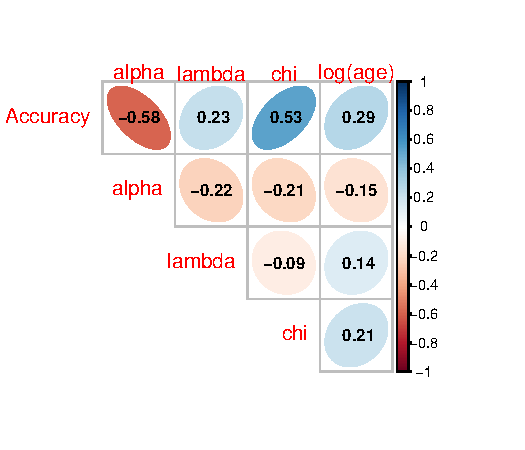
\includegraphics{figs/unnamed-chunk-1-1} \caption[Correlation of individuals' best-fitting model parameters with age and test accuracy]{Correlation of individuals' best-fitting model parameters with age and test accuracy. Accuracy is strongly related to higher learning rate (chi) and lower memory fidelity (alpha).}\label{fig:unnamed-chunk-1}
\end{figure}
\end{CodeChunk}

\begin{CodeChunk}
\begin{figure}[H]

{\centering 
\includegraphics{figs/fig1-perf-1} 

}

\caption[Participants' vs]{Participants' vs. model accuracy at test by age. The model generally matches participants' performance, except for outperforming 3-year-olds, who performed at chance (dotted line). Error bars show +/-1SE.}\label{fig:fig1-perf}
\end{figure}
\end{CodeChunk}

Figure 1 shows the correlations between participants' accuracy,
best-fitting model parameters, and log(age). All correlations are
significant (e.g., \(\lambda\) vs log(age) \(r = 0.14\),
\(t(187) = 1.99\), \(p<.05\)) except \(\lambda\) vs.~\(\chi\). Most
notable is that accuracy is strongly related to higher learning rate
\(\chi\) (\(r=0.53\)) and lower memory fidelity (\(\alpha=0.58\); better
learning is achieved by forgetting early, ambiguous evidence -- as has
been seen in other applications of this model), and only weakly related
to \(lambda\) (\(r=0.23\)) and age (\(r=0.29\)). Figure 3 shows
participants' best-fitting model parameters by age, revealing
developmental increases in learning rate (\(\chi\)) and attention to
uncertainty (\(\lambda\)), and decrease in memory fidelity (\(\alpha\)).
Children show greater individual differences, but on average match
adults' parameter values by age 8. A targeted analysis found that
children are more likely than adults to be familiarity-focused
(\(\lambda<1\)) rather than uncertainty-focused (\(\chi^2 = 7.41\)):
22\% of adults had \(\lambda<1\), while 41\% of children did.

\begin{CodeChunk}
\begin{figure}[H]

{\centering 
\includegraphics{figs/fig2-parms-1} 

}

\caption[Participants' best-fitting model parameters by age reveal developmental change]{Participants' best-fitting model parameters by age reveal developmental change: learning rate (chi) and attention to uncertainty (lambda) generally increase with age, while memory fidelity (alpha) decreases. Error bars show +/-1SE.}\label{fig:fig2-parms}
\end{figure}
\end{CodeChunk}

\subsection{Selection strategies}\label{selection-strategies}

Overall, entropy was the most common strategy (60\% of participants),
followed by margin sampling (18\%), confirmatory (12\%), random (8\%),
and novelty (3\%). Figure 4 shows the proportion of participants by age
group that are most likely to be using each selection strategy. Children
were more likely to use entropy maximization (84\% vs.~37\% of adults),
whereas adults were more likely to use a confirmatory strategy (22\%
vs.~3\% of children) or margin sampling (22\% vs.~14\% of children).
Random selection was most likely for only 13\% of adults and only 3\% of
children, and novelty was most likely for 5\% of adults and no children.

\subsection{Relative contributions of strategy, age, and learning
mechanisms}\label{relative-contributions-of-strategy-age-and-learning-mechanisms}

To assess the relative importance of sampling strategy versus learning
mechanisms in predicting performance, we fitted a series of nested
regression models. Sampling strategy was treatment-coded with
confirmatory sampling as the baseline. A model including only sampling
strategy explained minimal variance in test accuracy (\(R^2 = .02\),
F(4,185) = 0.94, \(p=0.44\)), demonstrating that strategy choice alone
is a weak predictor of learning success. In contrast, a full model
including strategy, age, and learning parameters (\(\chi\), \(\lambda\),
\(\alpha\)) explained substantial variance (\(R^2=0.58\),
\(F(8,180) = 30.59\), \(p<.001\)). Learning rate (\(\chi\):
\(\beta = 0.33\), \(p < .001\)), memory decay (\(\alpha\):
\(\beta = -0.65\), \(p < .001\)), and attention to uncertainty
(\(\lambda\): \(\beta = 0.01\), \(p = .002\)) were all significant
predictors, as was age (\(\beta = 0.08\), \(p = .002\)). Notably,
strategy effects emerged when controlling for individual differences in
learning mechanisms: entropy maximization (\(\beta = 0.14\), \(p=.007\))
and margin sampling (\(\beta = 0.14\), \(p=.02\)) significantly
outperformed confirmatory sampling. These findings indicate that
developmental improvements in word learning operate through measurable
changes in learning rate and memory, additional age-related factors not
captured by these parameters, and to a lesser extent through strategic
information-seeking choices.

\begin{CodeChunk}
\begin{figure}[tb]
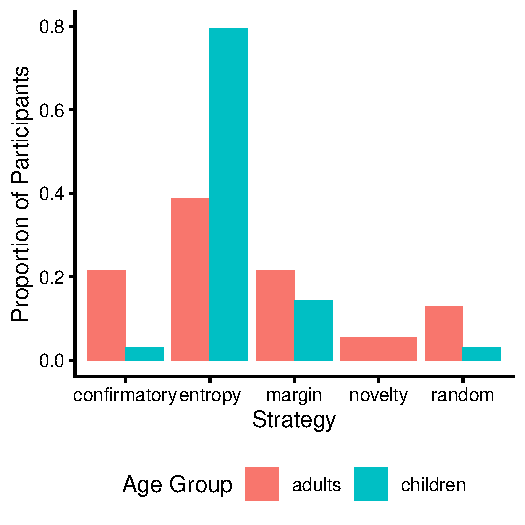
\includegraphics{figs/unnamed-chunk-6-1} \caption[Best-fitting selection strategies by age group]{Best-fitting selection strategies by age group. A higher proportion of children (vs. adults) used a entropy-based information gain strategy, while a higher proportion of adults used a confirmatory or margin sampling strategy.}\label{fig:unnamed-chunk-6}
\end{figure}
\end{CodeChunk}

\section{Discussion}\label{discussion}

We investigated the computational mechanisms underlying active word
learning by fitting associative learning models to individual
participants' performance and analyzing their information-seeking
strategies. Two models with uncertainty-biased attention best explained
learning for nearly all participants, with an uncertainty-only model
(UAM) best accounting for 51\% of individuals and the combined
familiarity-uncertainty model (FUAM) accounting for 48\%. This suggests
that directing attention toward uncertain associations (i.e., items with
diffuse mappings) is a fundamental mechanism in cross-situational word
learning in both adults and children. These two models -- differing only
in whether the current association strength is considered in the update
rule -- very nearly mimicked each other for the bulk of the
participants, but each model best explained a substantial group of
participants, suggesting some individual variability in learning styles.
Examining the best-fitting parameters showed that learning rate and
memory decay predicted performance more strongly than attention biases.
Participants with higher learning rates (\(\chi\)) and lower memory
fidelity (\(\alpha\); effectively forgetting early ambiguous evidence)
were more accurate at test. A relatively weak relationship between
\(\lambda\) (attention to uncertainty) and performance (\(r = 0.23\))
suggests that how much learners encode matters more than what they
attend to, at least in these experimental paradigms.

An analysis of selection strategies showed some developmental
differences, but also some consistency: Adults and children both
predominantly employed entropy maximization (39\% of adults; 84\% of
children), actively seeking information about ambiguous items to reduce
uncertainty. However, adults deployed more diverse strategies: 22\% used
confirmatory sampling (vs.~3\% of children), 22\% used margin sampling
(vs.~14\% of children), and 13\% used random selection (vs.~3\% of
children).

This pattern suggests that children robustly deploy
uncertainty-reduction strategies, consistent with broader findings on
the development of information-seeking in childhood (Meder et al., 2021;
Nussenbaum et al., 2020). The high prevalence of entropy maximization in
children aligns with evidence that young learners actively seek
information to resolve uncertainty across multiple domains (Liquin \&
Gopnik, 2022). However, adults' greater strategic diversity suggests
that development may involve not the emergence of uncertainty reduction
\emph{per se}, but rather the acquisition of a more flexible repertoire
of strategies that can be adaptively deployed depending on task demands
(Ruggeri et al., 2021). This flexibility may reflect adults' greater
metacognitive awareness of when uncertainty reduction is optimal versus
when alternative strategies (e.g., confirmation, exploitation) are more
efficient.

Why might children show less strategic diversity than adults, relying so
heavily on entropy maximization? One possibility is that children's
nascent metacognitive skills make it harder to flexibly shift between
different information-seeking strategies based on task context (Baer \&
Kidd, 2022; Eccher et al., 2024). Entropy maximization may be a robust
default strategy that works well across many learning contexts and
requires only tracking which items are most ambiguous. In contrast,
deploying confirmatory or margin sampling strategies effectively may
require greater metacognitive sophistication: recognizing when one's
current strongest hypothesis is worth testing (confirmation) or when
near-threshold distinctions matter most (margin sampling). Thus, adults'
strategic diversity may reflect the development of metacognitive
flexibility that allows adaptive strategy selection based on learning
goals and task structure (Ruggeri et al., 2021). Alternatively,
children's limited working memory may make it difficult to
simultaneously maintain multiple competing hypotheses and evaluate the
diagnosticity of different sampling strategies, leading them to default
to a single reliable approach (Zettersten, Choi, et al., 2025).

A central theoretical question is whether sampling ambiguous items
causes better learning, or whether successful learning enables more
sophisticated sampling strategies. Our results support the latter
interpretation. Learning parameters \(\chi\) and \(\alpha\) strongly
predicted performance, while sampling strategy showed weaker
relationships to outcomes. This finding aligns with Zettersten \&
Saffran (2021)'s supplementary analysis which suggested that
successfully learning novel words during training makes it more likely
that learners will subsequently focus on ambiguous items. We extend this
result by showing that individual differences in learning mechanisms
(learning rate, memory) are the primary drivers of both performance and
sampling sophistication. However, the current experimental design limits
our ability to test causality: selection trials occurred \emph{after}
initial learning, and we modeled them using associations built during
passive training. Future work using trial-by-trial joint optimization of
learning and selection parameters could better disentangle these
relationships.

Combining computational modeling of learning mechanisms with analysis of
selection strategies reveals a nuanced picture of active word learning
across development. Successful learning depends more on fundamental
learning parameters (i.e., how quickly associations form and how readily
early evidence is forgotten) rather than a bias to attend more or less
to uncertain (or already-familiar) items. However, the likelihood of
strategically sampling uncertain information emerges across childhood,
which may suggest an increasing awareness of uncertainty, or of the
value of reducing it. These findings advance our understanding of how
learners actively shape their own language learning experience, and how
cognitive development enables increasingly sophisticated
information-seeking strategies.

\section{Acknowledgements}\label{acknowledgements}

We thank the participants who enabled this research.

\section{References}\label{references}

\setlength{\parindent}{-0.1in} 
\setlength{\leftskip}{0.125in}

\noindent

\phantomsection\label{refs}
\begin{CSLReferences}{1}{0}
\bibitem[\citeproctext]{ref-baer_learning_2022}
Baer, C., \& Kidd, C. (2022). Learning with certainty in childhood.
\emph{Trends in Cognitive Sciences}, \emph{26}(10), 887--896.
\url{https://doi.org/10.1016/j.tics.2022.07.010}

\bibitem[\citeproctext]{ref-de_eccher_childrens_2024}
Eccher, M. de, Mundry, R., \& Mani, N. (2024). Children's subjective
uncertainty-driven sampling behaviour. \emph{Royal Society Open
Science}, \emph{11}(4), 231283.
\url{https://doi.org/10.1098/rsos.231283}

\bibitem[\citeproctext]{ref-gelderloos_active_2020}
Gelderloos, L., Mahmoudi Kamelabad, A., \& Alishahi, A. (2020). Active
word learning through self-supervision. In S. Denison, M. Mack, Y. Xu,
\& B. C. Armstrong (Eds.), \emph{Proceedings for the 42nd {Annual}
{Meeting} of the {Cognitive} {Science} {Society}} (pp. 1050--1056).
Cognitive Science Society.

\bibitem[\citeproctext]{ref-gureckis2012self}
Gureckis, T. M., \& Markant, D. B. (2012). Self-directed learning: A
cognitive and computational perspective. \emph{Perspectives on
Psychological Science}, \emph{7}(5), 464--481.
\url{https://doi.org/10.1177/1745691612454304}

\bibitem[\citeproctext]{ref-hembacher_childrens_2020}
Hembacher, E., DeMayo, B., \& Frank, M. C. (2020). Children's social
information seeking is sensitive to referential ambiguity. \emph{Child
Development}, \emph{91}(6), e1178--e1193.
\url{https://doi.org/10.1111/cdev.13427}

\bibitem[\citeproctext]{ref-Hidaka2017}
Hidaka, S., Torii, T., \& Kachergis, G. (2017). Quantifying the impact
of active choice in word learning. In G. Gunzelmann, A. Howes, T.
Tenbrink, \& E. Davelaar (Eds.), \emph{Proceedings of the 39th {Annual}
{Meeting} of the {Cognitive} {Science} {Society}} (pp. 519--525).
Cognitive Science Society.

\bibitem[\citeproctext]{ref-Kachergis2012}
Kachergis, G., Yu, C., \& Shiffrin, R. M. (2012). An associative model
of adaptive inference for learning word--referent mappings.
\emph{Psychonomic Bulletin and Review}, \emph{19}(2), 317--324.
\url{https://doi.org/10.3758/s13423-011-0194-6}

\bibitem[\citeproctext]{ref-kachergis2013actively}
Kachergis, G., Yu, C., \& Shiffrin, R. M. (2013). Actively learning
object names across ambiguous situations. \emph{Topics in Cognitive
Science}, \emph{5}(1), 200--213.
\url{https://doi.org/10.1111/tops.12008}

\bibitem[\citeproctext]{ref-Kachergis2017}
Kachergis, G., Yu, C., \& Shiffrin, R. M. (2017). A bootstrapping model
of frequency and contextual diversity effects in word learning.
\emph{Cognitive Science}, \emph{41}(3), 590--622.
\url{https://doi.org/10.1111/cogs.12353}

\bibitem[\citeproctext]{ref-Keijser2019}
Keijser, D., Gelderloos, L., \& Alishahi, A. (2019). Curious topics: {A}
curiosity-based model of first language word learning. \emph{Proceedings
of the 41st {Annual} {Conference} of the {Cognitive} {Science}
{Society}}, 1991--1997.

\bibitem[\citeproctext]{ref-liquin_children_2022}
Liquin, E., \& Gopnik, A. (2022). Children are more exploratory and
learn more than adults in an approach-avoid task. \emph{Cognition},
\emph{218}, 104940.
\url{https://doi.org/10.1016/j.cognition.2021.104940}

\bibitem[\citeproctext]{ref-markant2016}
Markant, D. B., Settles, B., \& Gureckis, T. M. (2016). Self-directed
learning favors local, rather than global, uncertainty. \emph{Cognitive
Science}, \emph{40}(1), 100--120.
\url{https://doi.org/10.1111/cogs.12220}

\bibitem[\citeproctext]{ref-meder_directed_2021}
Meder, B., Wu, M. C., Schulz, E., \& Ruggeri, A. (2021). Development of
directed and random exploration in children. \emph{Developmental
Science}, \emph{24}(4), e13095. \url{https://doi.org/10.1111/desc.13095}

\bibitem[\citeproctext]{ref-Nelson2005}
Nelson, J. D. (2005). Finding useful questions: {On} {Bayesian}
diagnosticity, probability, impact, and information. \emph{Psychological
Review}, \emph{112}(4), 979--999.
\url{https://doi.org/10.1037/0033-295X.112.4.979}

\bibitem[\citeproctext]{ref-nussenbaum_causal_2019}
Nussenbaum, K., Cohen, A. O., Davis, Z. J., Halpern, D., Gureckis, T.,
\& Hartley, C. (2020). Causal information-seeking strategies change
across childhood and adolescence. \emph{Cognitive Science},
\emph{44}(9), e12888. \url{https://doi.org/10.1111/cogs.12888}

\bibitem[\citeproctext]{ref-nussenbaum_novelty_2023}
Nussenbaum, K., Martin, R. E., Maulhardt, S., Yang, Y. J.,
Bizzell-Hatcher, G., Bhatt, N. S., Koenig, M., Rosenbaum, G. M.,
O'Doherty, J. P., \& Cockburn, J. (2023). Novelty and uncertainty
differentially drive exploration across development. \emph{Elife},
\emph{12}, e84260. \url{https://elifesciences.org/articles/84260}

\bibitem[\citeproctext]{ref-ruggeri_how_2021}
Ruggeri, A., Walker, C. M., Lombrozo, T., \& Gopnik, A. (2021). How to
{Help} {Young} {Children} {Ask} {Better} {Questions}? \emph{Frontiers in
Psychology}, \emph{11}. \url{https://doi.org/10.3389/fpsyg.2020.586819}

\bibitem[\citeproctext]{ref-Settles2012}
Settles, B. (2012). \emph{Active {Learning}} (Vol. 6).
\url{https://doi.org/10.2200/S00429ED1V01Y201207AIM018}

\bibitem[\citeproctext]{ref-smith2018developing}
Smith, L. B., Jayaraman, S., Clerkin, E., \& Yu, C. (2018). The
developing infant creates a curriculum for statistical learning.
\emph{Trends in Cognitive Sciences}, \emph{22}(4), 325--336.
\url{https://doi.org/10.1016/j.tics.2018.02.004}

\bibitem[\citeproctext]{ref-twomey2018curiosity}
Twomey, K. E., \& Westermann, G. (2018). Curiosity-based learning in
infants: A neurocomputational approach. \emph{Developmental Science},
\emph{21}(4), e12629. \url{https://doi.org/10.1111/desc.12629}

\bibitem[\citeproctext]{ref-wason1960}
Wason, P. C. (1960). On the failure to eliminate hypotheses in a
conceptual task. \emph{Quarterly Journal of Experimental Psychology},
\emph{12}(3), 129--140. \url{https://doi.org/10.1080/17470216008416717}

\bibitem[\citeproctext]{ref-woodard2016}
Woodard, K., Gleitman, L. R., \& Trueswell, J. C. (2016). Two-and
three-year-olds track a single meaning during word learning: Evidence
for propose-but-verify. \emph{Language Learning and Development},
\emph{12}(3), 252--261.
\url{https://doi.org/10.1080/15475441.2016.1140581}

\bibitem[\citeproctext]{ref-yu2007rapid}
Yu, C., \& Smith, L. B. (2007). Rapid word learning under uncertainty
via cross-situational statistics. \emph{Psychological Science},
\emph{18}(5), 414--420.
\url{https://doi.org/10.1111/j.1467-9280.2007.01915.x}

\bibitem[\citeproctext]{ref-ZetterstenChenWilliams2025}
Zettersten, M., Chen, J., \& Lew-Williams, C. (2025). Children explore
conservatively when learning novel word extensions. \emph{Proceedings of
the 47th {Annual} {Conference} of the {Cognitive} {Science} {Society}},
1307--1313.

\bibitem[\citeproctext]{ref-zettersten_active_2025}
Zettersten, M., Choi, K., Kirkorian, H., \& Saffran, J. (2025).
\emph{Active sampling helps children learn new words by tuning their
curriculum to past experiences} {[}Preprint{]}. PsyArXiv.
\url{https://doi.org/10.31234/osf.io/ne43k_v1}

\bibitem[\citeproctext]{ref-zettersten_active_2023}
Zettersten, M., Cutler, M., \& Lew-Williams, C. (2023). Active
information-seeking in support of learning extensions of novel words.
\emph{Proceedings of the 45th {Annual} {Conference} of the {Cognitive}
{Science} {Society}}, 3018--3024.

\bibitem[\citeproctext]{ref-Zettersten2021}
Zettersten, M., \& Saffran, J. R. (2021). Sampling to learn words:
Adults and children sample words that reduce referential ambiguity.
\emph{Developmental Science}, \emph{24}(3).
\url{https://doi.org/10.1111/desc.13064}

\end{CSLReferences}

\bibliographystyle{apacite}


\end{document}
